\documentclass[11pt,a4paper,oneside]{report}


\usepackage{amsmath,amssymb,calc,ifthen}

\usepackage{float}

\usepackage[table,usenames,dvipsnames]{xcolor} % for coloured cells in tables

\usepackage{tikz}

% Allows us to click on links and references!

\usepackage{hyperref}
\hypersetup{
    colorlinks,
    citecolor=black,
    filecolor=black,
    linkcolor=black,
    urlcolor=black
}

% Nice package for plotting graphs
% See excellent guide:
% http://www.tug.org/TUGboat/tb31-1/tb97wright-pgfplots.pdf
\usetikzlibrary{plotmarks}
\usepackage{amsmath,graphicx}
\usepackage{epstopdf}
\usepackage{caption}
\usepackage{subcaption}

% highlight - useful for TODOs and similar
\usepackage{color}
\newcommand{\hilight}[1]{}%\colorbox{yellow}{#1}}

\newcommand\ci{\perp\!\!\!\perp}

% margin size
\usepackage[margin=1in]{geometry}

\tikzstyle{state}=[circle,thick,draw=black, align=center, minimum size=2.1cm,
inner sep=0]
\tikzstyle{vertex}=[circle,thick,draw=black]
\tikzstyle{terminal}=[rectangle,thick,draw=black]
\tikzstyle{edge} = [draw,thick]
\tikzstyle{lo} = [edge,dotted]
\tikzstyle{hi} = [edge]
\tikzstyle{trans} = [edge,->]

\title{Graphical Models Coursework 1}
\author{
    Razvan Valentin Marinescu\\
    \texttt{razvan.marinescu.14@ucl.ac.uk}
    \and
    David Owen\\
    \texttt{email.address@ucl.ac.uk}
    \and
    Kin Quan\\
    \texttt{email.address@ucl.ac.uk}
}

\begin{document}
\belowdisplayskip=12pt plus 3pt minus 9pt
\belowdisplayshortskip=7pt plus 3pt minus 4pt

\maketitle{}


\section*{Problem 2.5}
Hello

\section*{Problem 2.6}


\section*{Problem 2.7}


\section*{Problem 2.9}


\section*{Problem 3.3}

\begin{itemize}
 \item $tuberculosis \ci smoking\;|\; shortness\;of\;breath$ is \textbf{false}, because path $t \to e \to d \to b \to s$ is not blocked
 \item $lung\;cancer \ci  bronchitis\;|\;smoking$ is \textbf{true}, because:
  \begin{itemize}
    \item path $l \to s \to b$ is blocked ($s$ is instantiated)
    \item path $l \to e \to d \to b$ is blocked (has collider ${e,d,b}$)
  \end{itemize}
 \item $visit \; to \; Asia \ci smoking\;|\;lung\;cancer$ is \textbf{true}, because:
   \begin{itemize}
    \item path $a \to t \to e \to l \to s$ is blocked ($l$ is instantiated)
    \item path $a \to t \to e \to d \to b \to s$ is blocked ($d$ is uninstantiated)
  \end{itemize}
 \item $visit \; to \; Asia \ci smoking\;|\;lung \; cancer; \; shortness \; of \; breath$ is \textbf{false} because path $a \to t \to e \to d \to b \to s$ is not blocked ($d$ is instantiated).
\end{itemize}



\section*{Problem 3.4}


\section*{Problem 3.8}


\section*{Problem 3.9}

\subsection*{1. Belief network}

\begin{figure}[H]
  \centering
    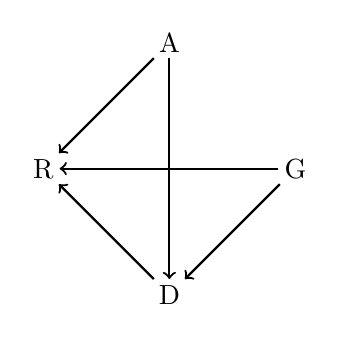
\begin{tikzpicture}[scale=0.8,help lines/.style={color=lightgray,line width=0.2pt},post/.style={->,shorten >=1pt,>=stealth',thick}]
    
    \node[inner sep=2] (A) at (0.0,2.0){A};
    \node[inner sep=2] (G) at (2.0,0.0) {G};
    \node[inner sep=2] (R) at (-2.0,0.0) {R};
    \node[inner sep=2] (D) at (0.0,-2.0) {D};

    \draw[->, thick] (A) -- (R);
    \draw[->, thick] (A) -- (D);
    \draw[->, thick] (G) -- (D);
    \draw[->, thick] (G) -- (R);
    \draw[->, thick] (D) -- (R);
    
    \end{tikzpicture}
    \caption{Belief network}
    \label{fig:all_trade_cca_black}     
\end{figure}

\subsection*{2. Computation of $p(recover \; | \; drug)$}

Applying Bayes rule we get $p(recover \; | \; drug) = \frac{p(recover, \;drug)}{p(drug)}$. This suggests that from a database of patient entries we take the number of patients that both recovered and received the drug and divide it by the number of patients that received the drug. 

\subsection*{2. Computation of $p(recover \; | \; do(drug),\; yound)$}

\section*{Problem 3.11}


\section*{Problem 3.12}


\section*{Problem 3.13}


\section*{Problem 3.14}


\section*{Problem 3.15}


\section*{Problem 3.17}

\subsection*{1.}

In order to prove $a \ci c$ we need to show that $p(a,c) = p(a)p(c)$. We first calculate the joint probability distribution $p(a,b,c) = p(c|b)p(b|a)p(a)$. Then we marginalise over $b$ to get $p(a,c)=\sum_{b} p(a,b,c) = \sum_{b} p(c|b)p(b|a)p(a)$. 

For $b=b_1$ we get $p(b1|a) = \left( \frac{1}{4} \frac{15}{40} \right)$

\section*{Problem 3.20}


\section*{Problem 3.21}


\section*{Problem 3.22}


\section*{Extra Problem A}


\section*{Extra Problem B}


\end{document}
